\section{Results} \label{sec:results}

In this section, we discuss our main results, primarily focusing on how well various \judgemodels are aligned with humans (\cref{sec:results:exploringhumanjudgellmalignment}) and how that impacts their usability (\cref{sec:results:exploringsystematicpatterns}).
To do so, we consider their Cohen's kappa coefficient \citep{cohen1960kappa}, and assess how differently they rank the nine \evaluatormodels of for which we computed benchmark results.
In \cref{sec:analysis}, we further analyse their precision and recall and dig deeper on the types of errors that various \judgemodels make.
% \subsection{How well are various judges aligned with humans?}

\subsection{Human - \JudgeModel Alignment}\label{sec:results:exploringhumanjudgellmalignment}

First, we compute the percentage alignment as well as Cohen's Kappa coefficient (kappa) between the evaluations of each \Judgemodels and human annotators for all \evaluatormodels. 
% We show both in \cref{fig:llmalignment}. 
In \cref{fig:llmalignment}, we see that while alignment is poor for most \judgemodels, both \judge{Llama3 70B} \citep{meta2024llama3} and \judge{GPT-4} \citep{achiam2023gpt} have kappa values that are considered to indicate excellent alignment (79 and 84\%, respectively).
Nevertheless, there still is a significant disparity between human judgment and \judgemodels. 
Even though judges with kappa > 80\% are considered perfectly aligned with human judgement, \judge{GPT-4} is still  12\% behind human judgement. 
Notably, classical lexical matching techniques like \judge{Contains} have higher kappa scores than half of \judgemodels. 

\paragraph{Kappa vs percent alignment}
Furthermore, by examining the error plots illustrated in \cref{fig:llmalignment}, it becomes evident that as judges deviate further from human judgments, there is an increase in variability in their kappa scores. 
When assessing judges' performance based on alignment percentage, there's merely a 30\% variance between human judgment and EM, whereas kappa indicates a 53\% disparity. 
Kappa scores more accurately reflect the declining trends in \judgemodels compared to alignment percentage, as illustrated by the instance where alignment percentage ranks \eval{Gemma 2B} higher than Kappa.
% \dieuwke{We should say something about the difference between percent alignment and Cohen's Kappa Coefficient (also can we shorten that, peraphs to CKC?)}

% We compute the Kappa score between the evaluations of each judge LLM and human annotation for all the evaluation models. From Figure \ref{fig:llmalignment}, we can see that judge llms significantly diverge from human judgement. Even though Judges with Kappa > 80\% are considered perfectly aligned with Human Judgement, GPT-4 is still 12\% behind human judgement. Notably, classical lexical matching techniques like Contains have higher Kappa scores than half of Judge LLMs.

 % Analysis depicted in Figure (cite LLM alignment fig) indicates that all Judge LLMs significantly diverge from human alignment, with even the state-of-the-art GPT-4 falling short by approximately 13\%. Notably, a simple contains keyword matching approach outperformed five out of twelve Judge models in aligning with human judgment. 


\begin{figure}[h]
    \centering
    \begin{subfigure}[b]{0.49\textwidth}
        \centering
        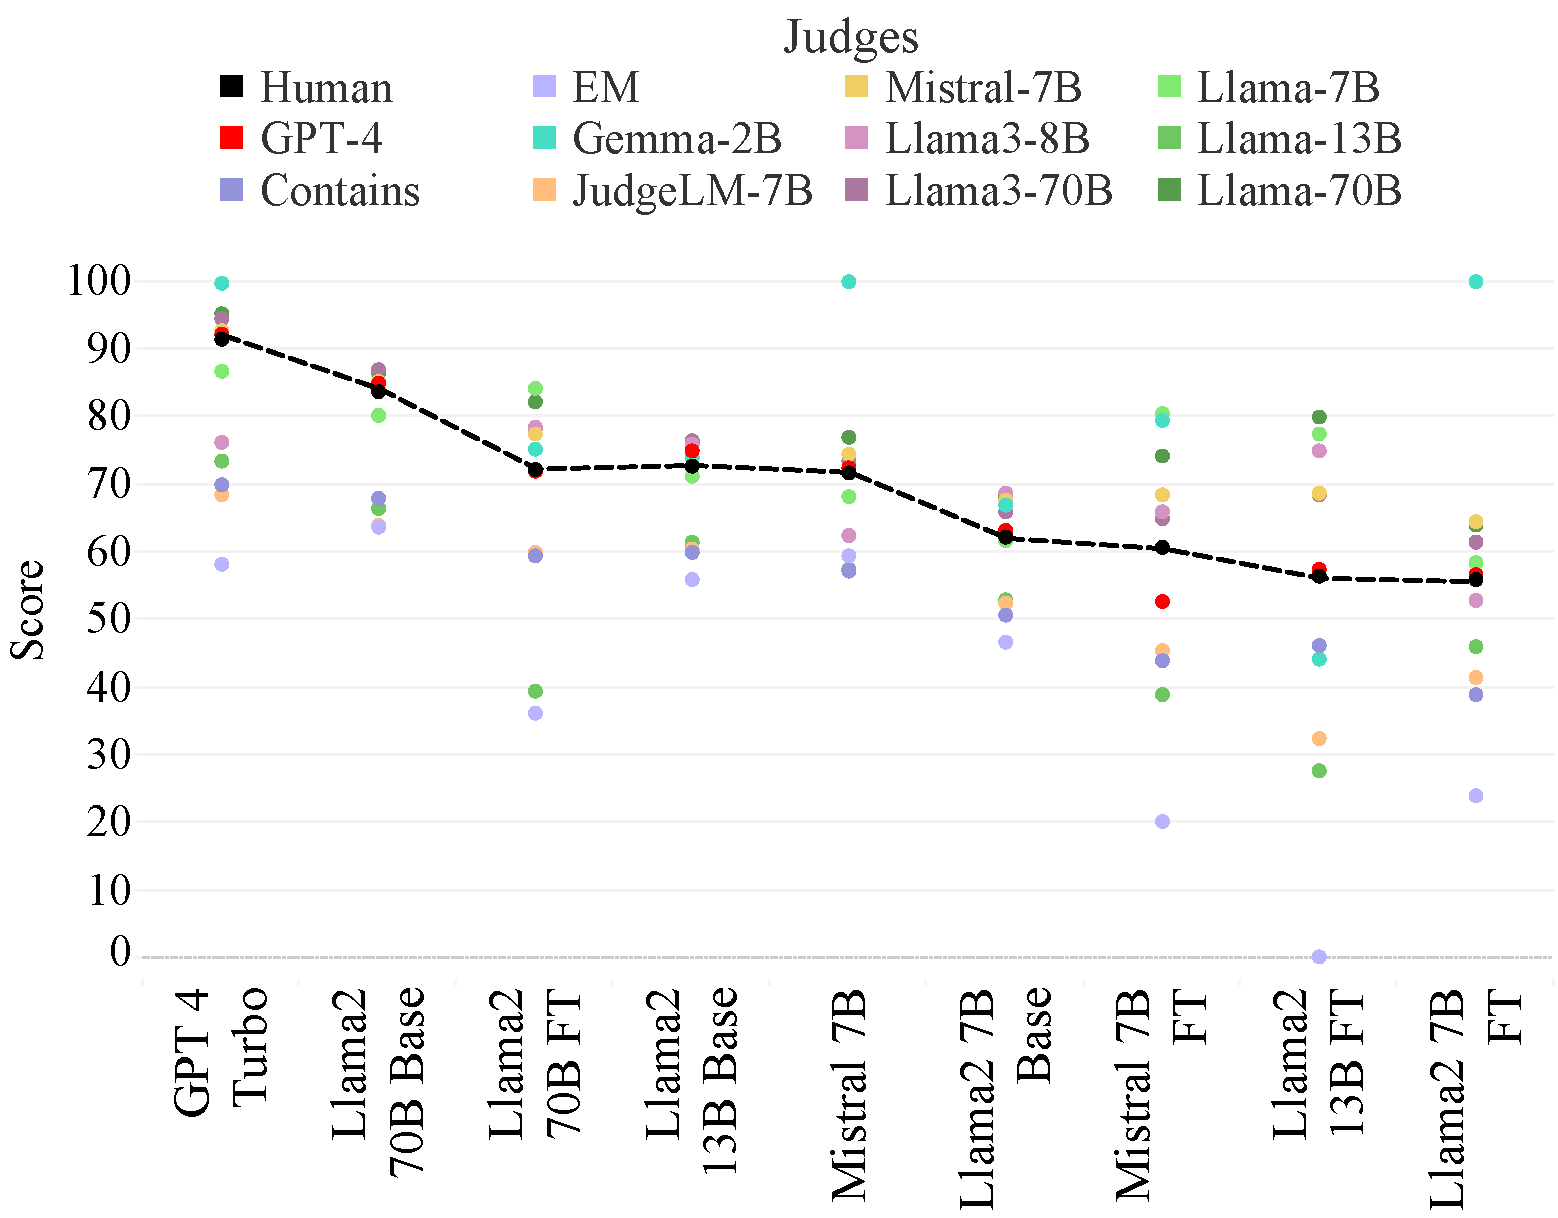
\includegraphics[width=\linewidth]{figures/JudgeScoreforExamTakers.pdf}
        \caption{}
        \label{fig:llmalignment_a}
    \end{subfigure}
    \hfill
    \begin{subfigure}[b]{0.49\textwidth}
        \centering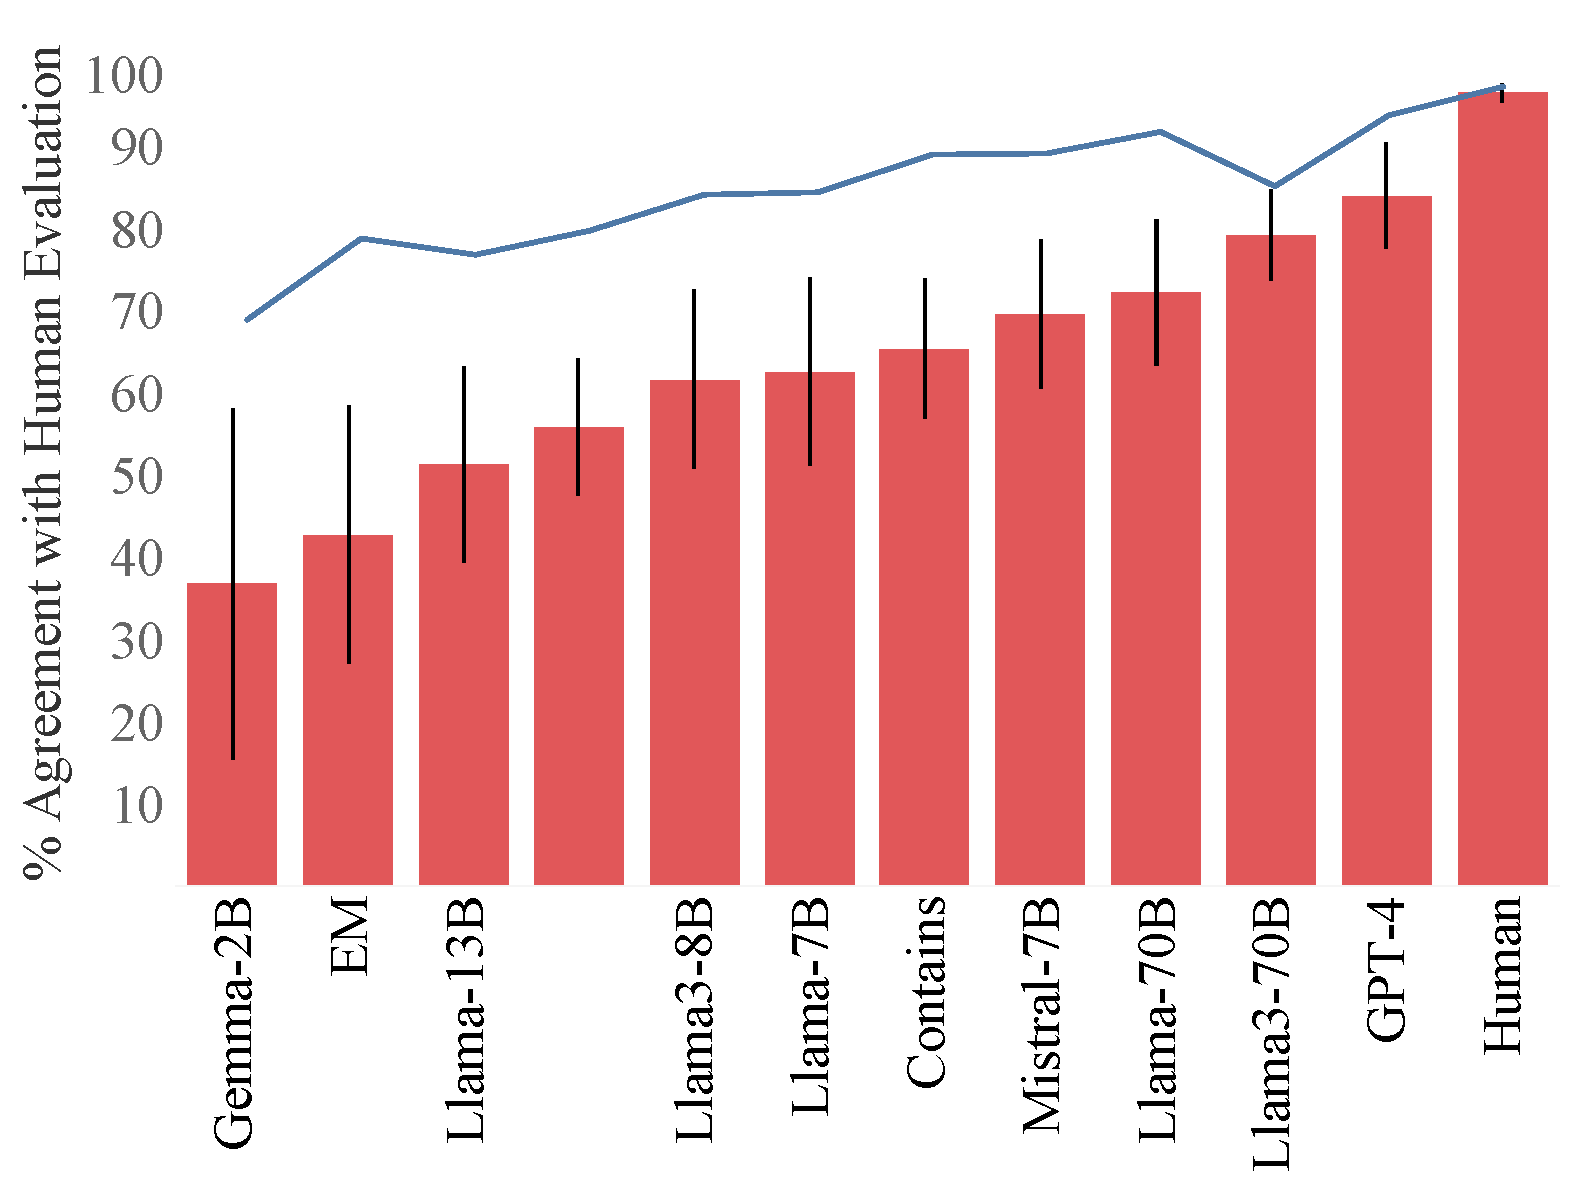
\includegraphics[width=\linewidth]{figures/LLMAlignmentV5.pdf}
        \caption{}
        \label{fig:assigned_scores}
    \end{subfigure}
    \caption{\Judgemodel alignment with human judgment, averaged across \textit{evaluatormodels}. The blue line indicates the percentage of aligned examples, the red bars Cohen's Kappa. 
    Error bars annotate standard deviation across \textit{evaluatormodels}. While alignment is poor for most \Judgemodel, both Llama3 70B and GPT 4 have Cohen's Kappa coefficient that are indicative of excellent alignment (79 and 84\%, respectively). Both of them, however, are still well below the human alignment score, which is 96\%.}
    \label{fig:llmalignment}
\end{figure}





% \subsubsection{Kappa Score vs Evaluation Score}

\paragraph{Kappa vs score}
To get a better idea of how much variation in actual assigned scores can be expected given a particular kappa, we plot the differences between scores provided by judges and those from human assessment across a range of judge kappa scores, in \cref{fig:cohenskappa}.
% \dieuwke{TODO: make y-axis log-scale}.
We can see that for Kappa > 80\%, the evaluation scores of \judgemodels are close to the human evaluation scores for most of the judges, with only up to 5\% difference in their assigned score.
For moderate or slight alignment, we observe a variation of up to 20\% in the evaluation scores for similar kappa alignment.
Furthermore, for several \judgemodels, we observe that the deviation from human-judgements can be quite different for different \evaluatormodels.
In \cref{fig:assigned_scores}, Gemma-2B, for instance, sometimes assigns higher scores than humans, an sometimes much lower.
In the next section, we further explore this particular topic.
\begin{figure}[h]
    \centering
    \begin{subfigure}[b]{0.4\textwidth}
        \centering
        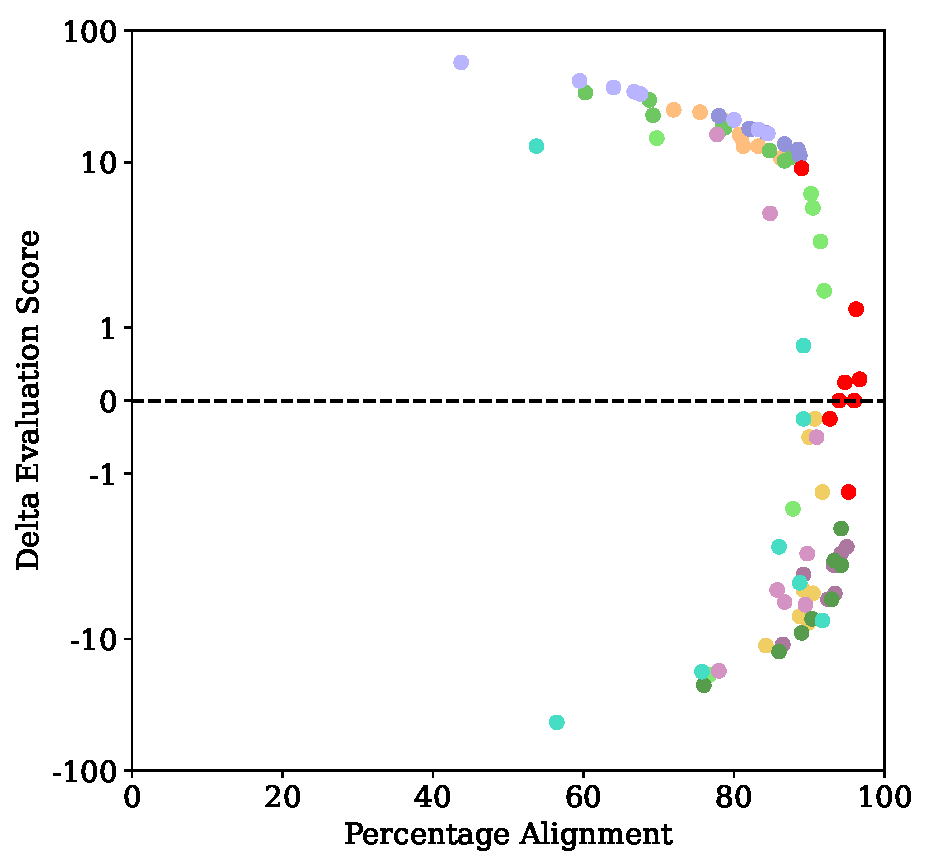
\includegraphics[width=\linewidth]{figures/KappaScoreVariation_V5_a.pdf}
        \caption{}
        \label{fig:cohenskappa_part1}
    \end{subfigure}%
    \begin{subfigure}[b]{0.6\textwidth}
        \centering
        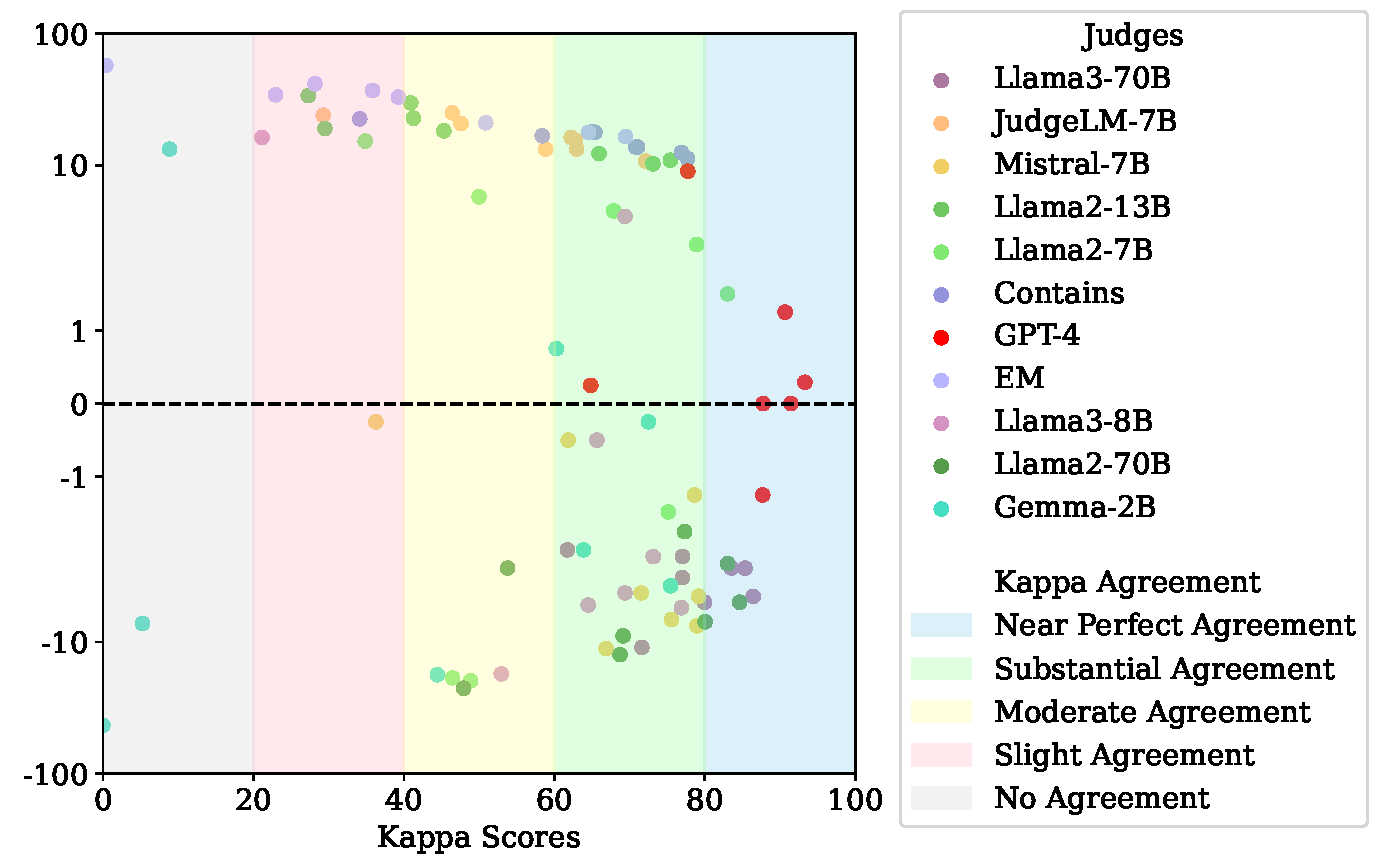
\includegraphics[width=\linewidth]{figures/KappaScoreVariation_V5_b.pdf}
        \caption{}
        \label{fig:cohenskappa_part2}
    \end{subfigure}
    \caption{Delta evaluation score is calculated by taking judge score difference with human judgement. In fig a), we observe skewed distribution for percentage alignment and delta evaluation score while in fig b) we observe that highly aligned LLM judges with kappa > 0.8 exhibit low score variance. Conversely, judges with kappa < 0.8 demonstrate variation, impacting reliability. }
    \label{fig:cohenskappa}
\end{figure}

% \subsection{How does this impact their usability?}
\subsection{Exploring Systematic Patterns in \JudgeModels} \label{sec:results:exploringsystematicpatterns}

% \begin{figure}[h]
%     \centering
%     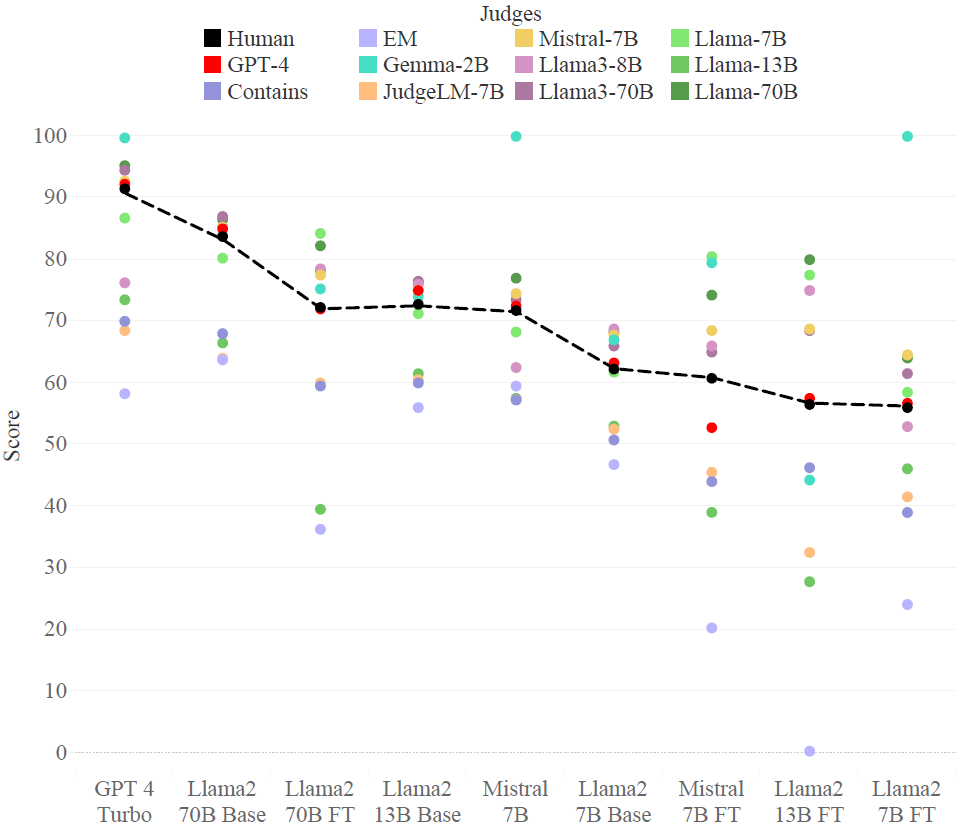
\includegraphics[width=\linewidth]{figures/JudgeScoreforExamTakers.png}
%     \caption{ We plot the delta between Judge exam scores and human assessment for various exam takers.Judge LLMs exhibit diverse distributions and rankings across different exam-taker, none of which exactly mirror the assessments of human judges. However, well aligned tend to consistently score more than the human assessment. \dieuwke{Invert this so that i) the exam taker models are on the y-axis, and the colour indicates the judges, and ii) put the actual score, not the delta.} \dieuwke{Potentially: put next to the figure with the rankings.}}
%     \label{fig:assigned_scores}
% \end{figure}

In the previous section, we have seen that none of the \judgemodels we considered were aligned as well with humans as humans themselves.
Furthermore, as can be seen in \cref{fig:assigned_scores}, the scores assigned by even the best aligned \judgemodels can differ up to 10 points with the human-assigned scores.
However, while this may limit -- to some extent -- the utility of using a \judgemodels to get a perfect estimate of how many of the questions the \evaluatormodels can answer perfectly, the \judgemodels may still offer valuable insights to \emph{differentiate} between different \evaluatormodels.
If judges exhibit systematic biases, such as consistently rating any \evaluatormodel lower -- akin to a very strict teacher -- they will not assign identical scores, but they may assign identical \emph{rankings}.

To evaluate this, we compare the rankings assigned by each \judgemodels to the nine \evaluatormodels (displayed in \cref{fig:rankcorrelation}) and compute their correlation with the human standard. 
In our analysis, it appears that the \eval{Contains} judge demonstrates the highest alignment with a Spearman's rank correlation coefficient ($\rho$) \citep{spearman1904spearman}, maintaining rank consistency across 6 out of 9 examined models. 
Notably, \eval{Contains} performs on par with JudgeLM-7B \citep{zhu2023judgelm}, a language model fine-tuned specifically for evaluating language model responses. 
Following closely behind, GPT-4 and Llama3-70B emerge as the second-best performers. 
Remarkably, while GPT-4 and Llama3 rank the same three models in positions three, four, and five as the human judge, they do so in different orders. 
Despite most judges exhibiting correlations ($\rho$) > 0.7 (\cref{app:correlationcoefftable}), they appear to struggle more in distinguishing between poorer-performing \evaluatormodels compared to better-performing ones.
% We see that all best-aligning judges are consistent in their ranking of the top two models: they all agree that, of the models evaluated, GPT4 is the best performing model, followed by Llama2-70b-base.
% Below the top two, there are more changes.
% The GPT-4 and Llama3 have the same three models in spot three, four and five as the human judge, but both with different orders.
% Generally, judges appear worse at distinguishing poorer performing models than better-performing models.

% Classical lexical models fare even worse with greater misalignment with human judgement across the board, with the -- commonly used -- EM score not even agreeing on the top-performing model.


% \begin{table}[h]
%     \centering
%     \begin{tabular}{|c|c|}
%     \hline
%     \textbf{Model} & \textbf{Spearman Rank Correlation Coeff} \\
%     \hline
%     Human Alignment & 100 \\
%     GPT-4 & 99.17 \\
%     Llama3-70B & 99.17 \\
%     Llama-70B & 81.67 \\
%     Mistral-7B & 77.50 \\
%     Contains & 41.67 \\
%     Llama-7B & 85.00 \\
%     Llama3-8B & 42.50 \\
%     JudgeLM-7B & 59.17 \\
%     Llama-13B & 18.33 \\
%     EM & 65.83 \\
%     Gemma-2B & 48.33 \\
%     \hline
%     \end{tabular}
%     \caption{Judges sorted by Kappa Human Alignment and their Spearman Rank Correlation Coeff}
%     \label{tab:scores_multiplied}
% \end{table}
\begin{figure}[h]
    \centering
    \begin{minipage}[b]{0.44\textwidth}
        \centering
        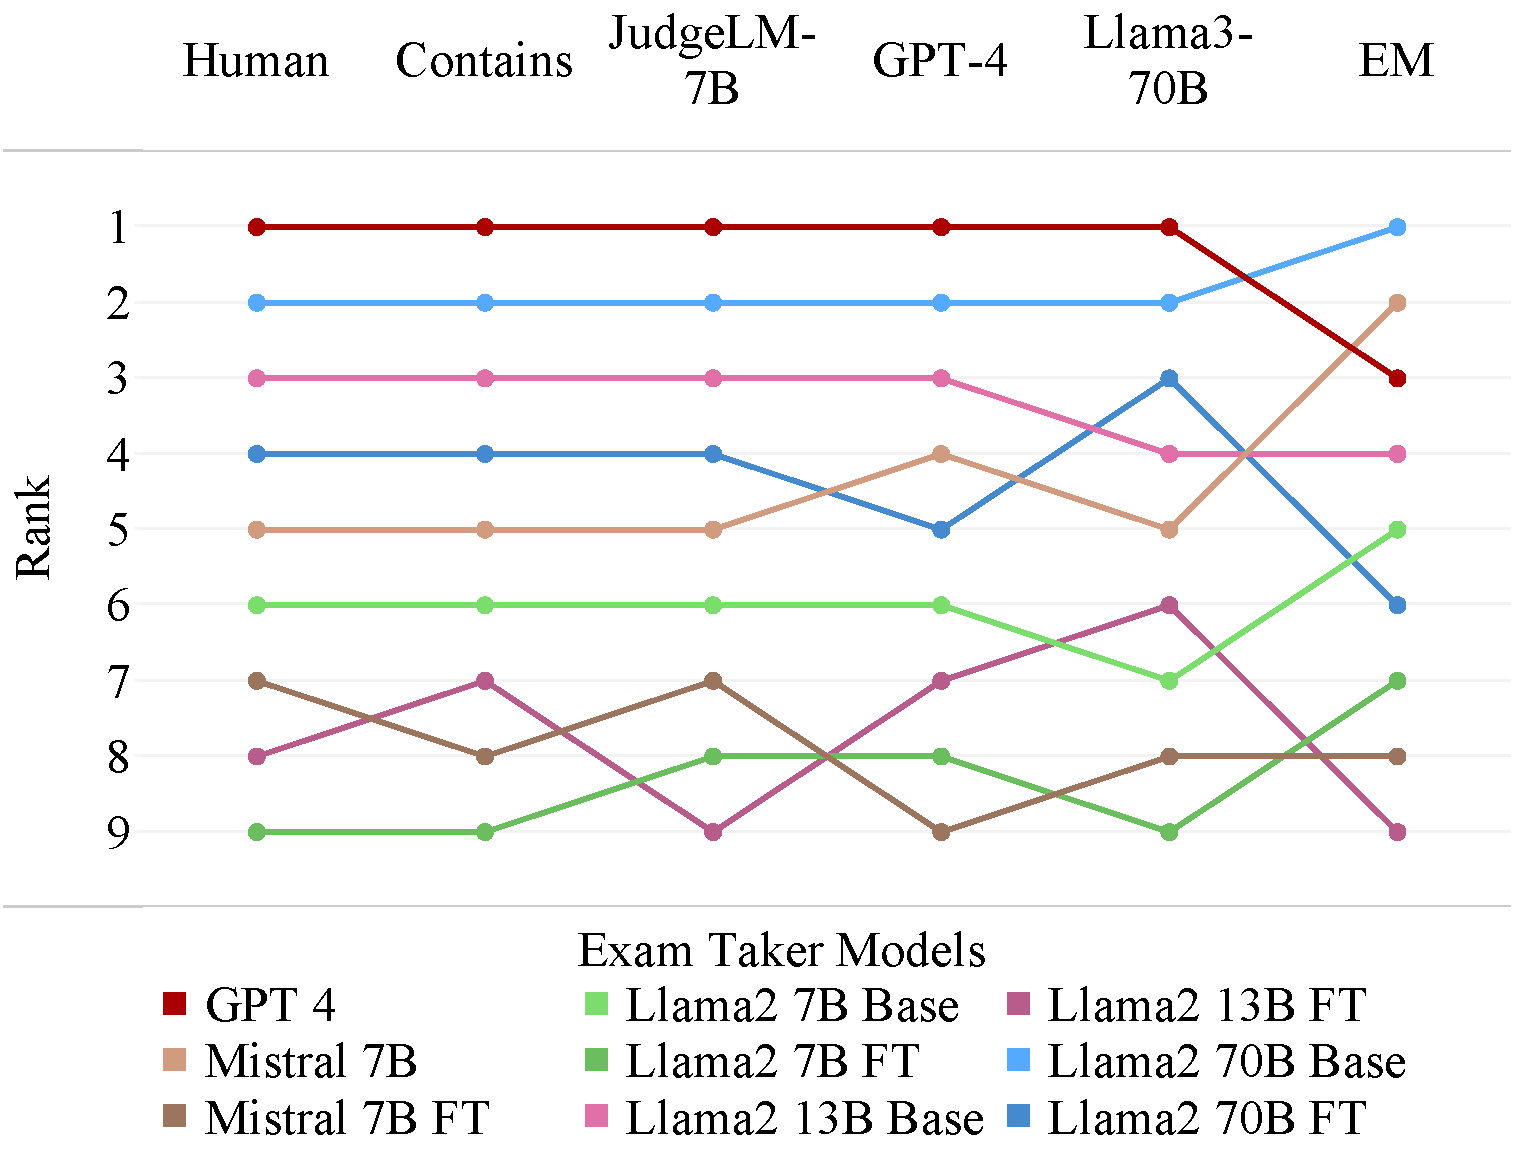
\includegraphics[width=\linewidth]{figures/RankOfEvaluationModels_V3.pdf}
        \caption{\eval{Contains} and \eval{JudgeLM} holds strong with a 67\% Human Assessment ranking retention, closely followed by GPT-4 and LLama3-70B. Notably, distinguishing between poor performing exam taker models presents a challenge for judges across the board}
        \label{fig:rankcorrelation}
    \end{minipage}
    \hfill
    \begin{minipage}[b]{0.54\textwidth}
        \centering
        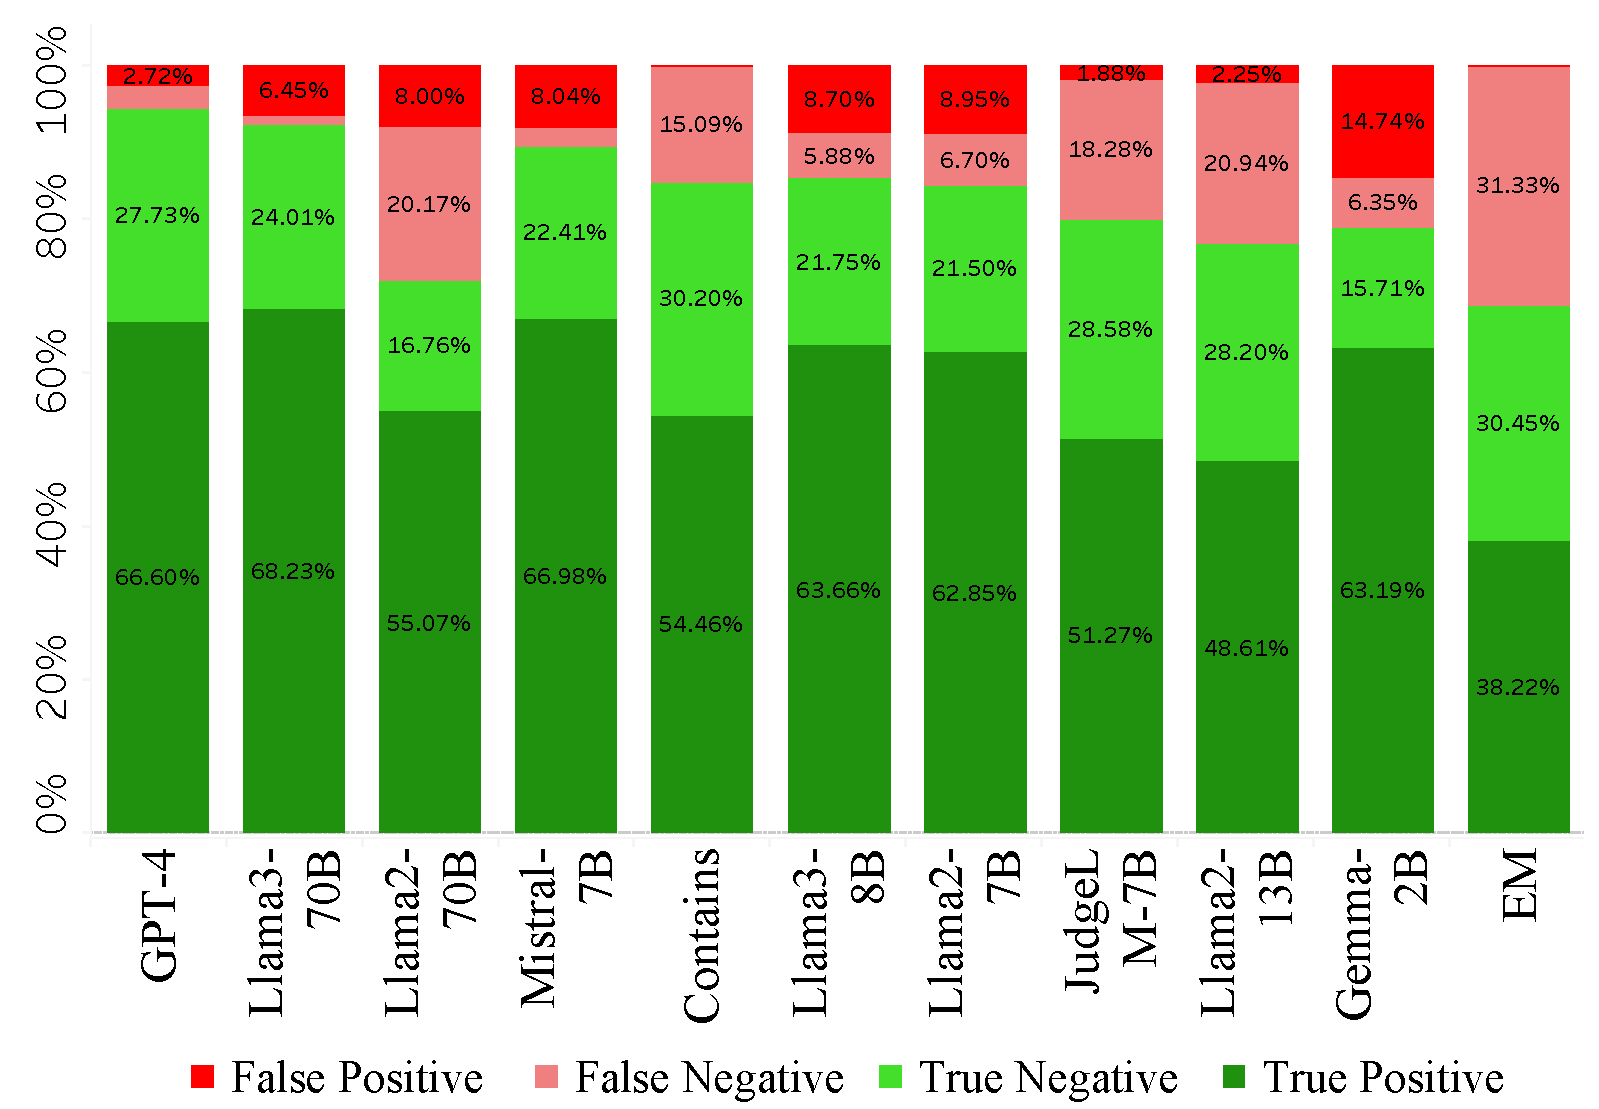
\includegraphics[width=\linewidth,height=5.7cm]{figures/ConfusionMatrixV4.pdf}
        \caption{false positives and negatives across different \judgemodels, ordered from best human aligned (left) to least human aligned (right). Generally, as alignment decreases, both FN and FP increase. Well-aligned models, however, tend to produce more FN than FP.
        \dieuwke{Should increase the font sizes on this one, put the legends on the top and afterwards align appropriately.}}
        \label{fig:confusionmatrix}
    \end{minipage}
\end{figure}


% \begin{figure}[h]
%     \centering
%     \begin{minipage}[b]{0.49\textwidth}
%         \centering
%         \includegraphics[width=\linewidth]{figures/InterLLMAlignment.png}
%         \caption{Inter Judge Alignment}
%         \label{fig:interllmalignment}
%     \end{minipage}
%     \hfill
%     \begin{minipage}[b]{0.49\textwidth}
%         \centering
%         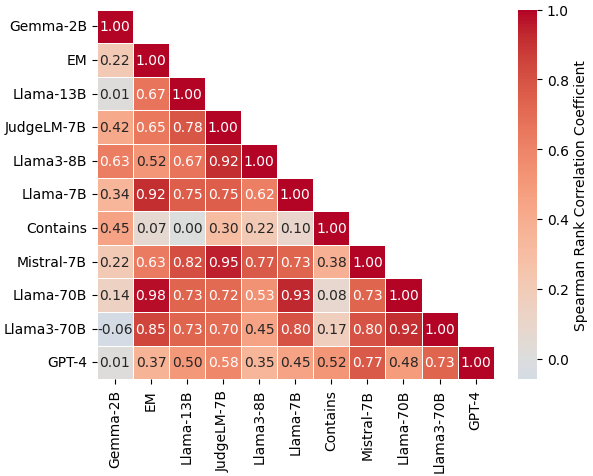
\includegraphics[width=\linewidth]{figures/RankCorrelationCoeff.png} 
%         \caption{Judge Ranking over Evaluation Models}
%         \label{fig:rankcorrelation}
%     \end{minipage}
% \end{figure}

% \subsubsection{Precision, Recall \& False Positives}

% Using the human judgement, we calculate the precision, recall and false positive rate to quantify judge LLM performance. To understand the precision-recall tradeoff, we plot the precision and recall rates and maintain The ordering of LLMs from Figure \ref{fig:llmalignment}. We can observe in figure \ref{fig:precisionrecall}, when LLMs become more aligned with human judgment, their recall improves. Precision, on the other hand, remains relatively consistent across all LLMs due to balancing effect of increase in true positive and false positives. From figure \ref{fig:confusionmatrix}, we can observe increase in true positives but not a similar reverse trend in False Positive. Instead, we see that the False Negatives are decreasing with increase in human alignment for Judges. 

% \begin{figure}[h]
%     \centering
%     \begin{minipage}[b]{\textwidth}
%         \centering
%         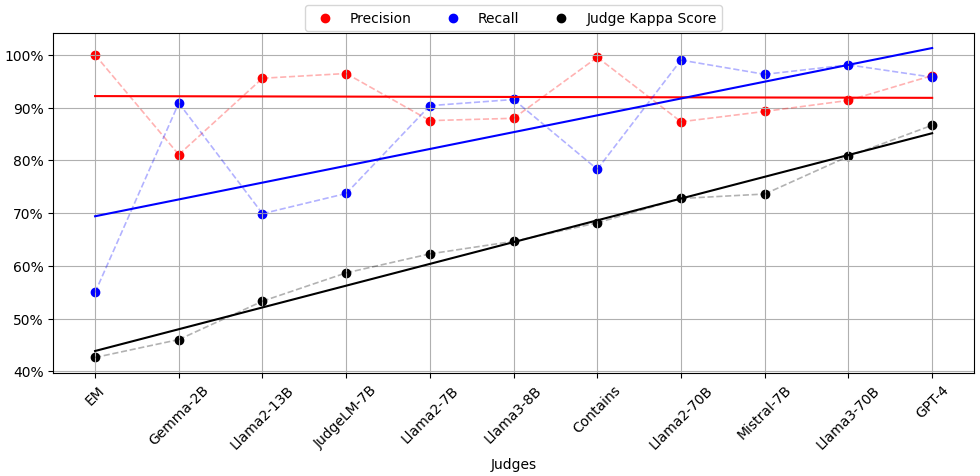
\includegraphics[width=\linewidth]{figures/PrecisionRecall_V4.png}
%         \caption{Precision \& recall with increasing human alignment}
%         \label{fig:precisionrecall}
%     \end{minipage}
% \end{figure}

% \begin{figure}[h]
%     \centering
%     \begin{minipage}[b]{\textwidth}
%         \centering
%         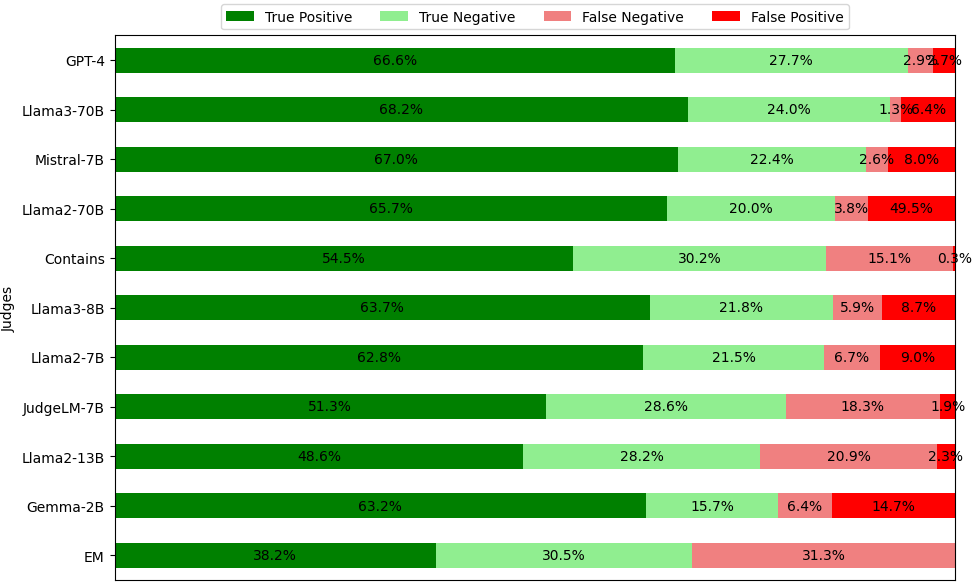
\includegraphics[width=\linewidth]{figures/ConfusionMatrixV2.png}
%         \caption{Judge performance \& error rate with increasing human alignment }
%         \label{fig:confusionmatrix}
%     \end{minipage}
% \end{figure}




% To explore the variability in scores among LLMs within the same cluster, we focus on the first group comprising Llama2-80B, Llama3-80B, Mistral-7B, and GPT-4, plotting their evaluation scores. Figure Y illustrates that despite similar Kappa scores for identical questions and evaluation models, judges' responses yield disparate evaluator results. In the worst-case scenario, these results can differ by up to 10 points

% \begin{figure}[h]
%     \centering
%     \begin{minipage}[b]{\textwidth}
%         \centering
%         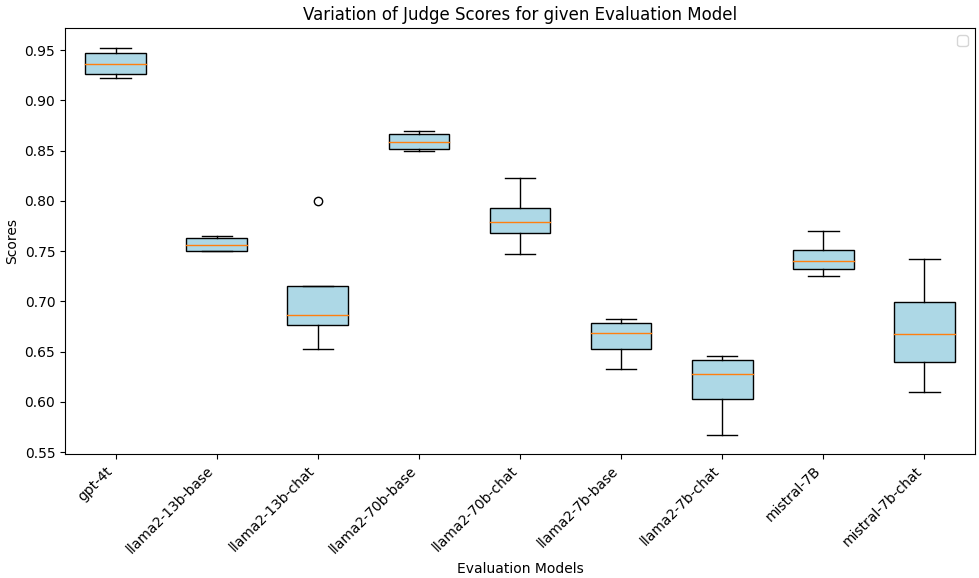
\includegraphics[width=\linewidth]{figures/VariationofScores.png}
%         \caption{Variation of Scores for similar Kappa Scores}
%         \label{fig:llmalignment}
%     \end{minipage}
% \end{figure}

% In our study, we investigated nine evaluation models and anticipated consistency in the ranking of judges across each model. To verify this assumption, we assessed the ranking of each judge across the different evaluation models. Recognizing the possibility of unchanging rankings (no variance), we computed and plotted the Spearman Rank Correlation Coefficient (cite) across the 12 judges. Spearman Rank Correlation is valuable as it gauges the degree to which the relationship between two variables can be described using a monotonic function. A Spearman Rank Correlation exceeding 0.7 indicates a strong correlation, a common occurrence in robust benchmarks. However, the plotted data in Figure (cite) reveals fluctuations in rankings among the remaining evaluators.

% \begin{figure}[h]
%     \centering
%     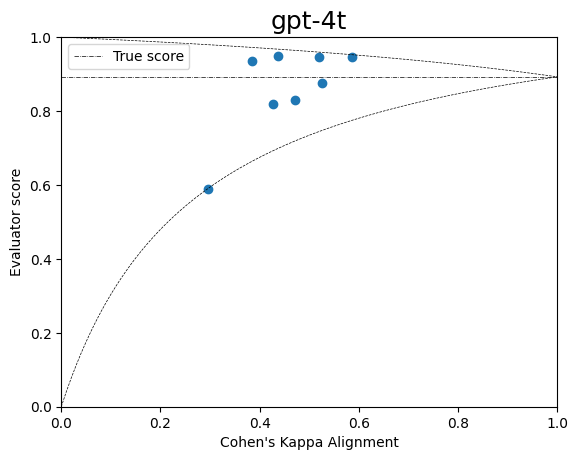
\includegraphics[width=0.6\textwidth]{figures/score-kappa-0.png}
%     \caption{Scores assigned by different evaluators vs their alignment with human evaluations}
%     \label{fig:score-kappa-0}
% \end{figure}

% \begin{figure}[h]
%     \centering
%     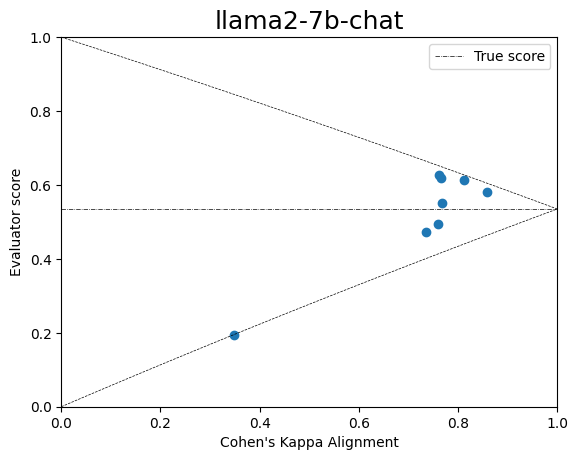
\includegraphics[width=0.6\textwidth]{figures/score-kappa-1.png}
%     \caption{Scores assigned by different evaluators vs their alignment with human evaluations}
%     \label{fig:score-kappa-0}
% \end{figure}

% \begin{figure}[h]
%     \centering
%     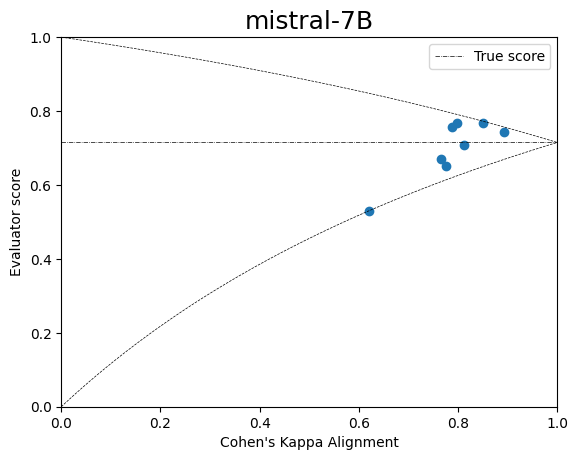
\includegraphics[width=0.6\textwidth]{figures/score-kappa-2.png}
%     \caption{Scores assigned by different evaluators vs their alignment with human evaluations}
%     \label{fig:score-kappa-0}
% \end{figure}





% OLD STUFF


% \begin{figure}[h]
%     \centering
%     \includegraphics[width=\textwidth]{figures/humanalignment_withem.png}
%     \caption{Human Alignment w GT}
%     \label{fig:human}
% \end{figure}

% \begin{table}[h]
%     \centering
%     \caption{Percentage Alignment}
%     \label{tab:my_table}
%     \begin{tabular}{cccccc}
%         \toprule
%         \textbf{Scenario} & \textbf{Avg Alignment} & \textbf{Human-A} & \textbf{Human-S} & \textbf{Human-K} & \textbf{Avg Size} \\
%         \midrule
%         All Questions & 98.33 & 97.33 & 98.5 & 99.17 & 600 \\
%         Low Confidence & 98.92 & 99.51 & 97.7 & 99.53 & 214 \\
%         High Confidence & 98.05 & 96.22 & 98.95 & 98.96 & 386 \\
%         \bottomrule
%     \end{tabular}
% \end{table}

% \begin{table}[htbp]
%     \centering
%     \begin{tabular}{cccccc}
%         \toprule
%         \textbf{Scenario} & \textbf{Avg Alignment} & \textbf{Human-A} & \textbf{Human-S} & \textbf{Human-K} & \textbf{Avg Size} \\
%         \midrule
%         All Questions & 96.75 & 94.81 & 97.08 & 98.38 & 308 \\
%         Low Confidence & 98.92 & 99.51 & 97.71 & 99.53 & 214 \\
%         High Confidence & 92.34 & 85.71 & 95.56 & 95.74 & 94 \\
%         \bottomrule
%     \end{tabular}
%     \caption{Without EM - Percentage Alignment}
%     \label{tab:my_table2}
% \end{table}

% \begin{table}[htbp]
%     \centering
%     \caption{Kappa Scores}
%     \label{tab:my_table2}
%     \begin{tabular}{cccccc}
%         \toprule
%         \textbf{Scenario} & \textbf{Avg Kappa} & \textbf{Human-A} & \textbf{Human-S} & \textbf{Human-K} & \textbf{Avg Size} \\
%         \midrule
%         All Questions & 96.36 & 94.14 & 96.75 & 98.19 & 600 \\
%         All Questions - EM & 92.38 & 88.06 & 92.96 & 96.13 & 600 \\
%         \bottomrule
%     \end{tabular}
% \end{table}

% \begin{figure}[h]
%     \centering
%     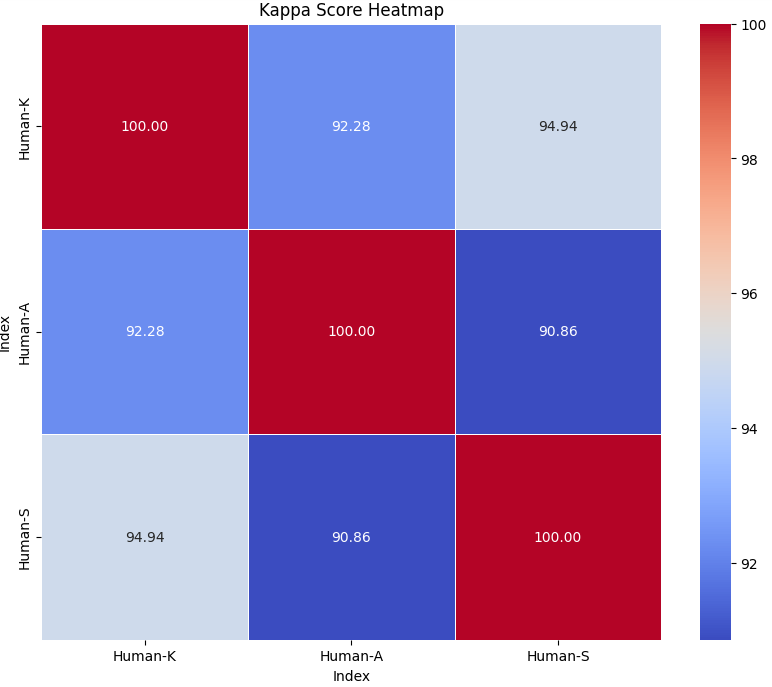
\includegraphics[width=0.8\textwidth]{figures/HumanHeatMap.png}
%     \caption{Human Alignment with Kappa Scores}
%     \label{fig:human}
% \end{figure}
